
\documentclass[12pt,a4paper]{article}

\usepackage{pdflscape}
\setlength{\textwidth}{165mm}
\setlength{\textheight}{235mm}
\setlength{\oddsidemargin}{-0mm}
\setlength{\topmargin}{-10mm}

\usepackage{mathtools}
\DeclarePairedDelimiter\abs{\lvert}{\rvert}%
\DeclarePairedDelimiter\norm{\lVert}{\rVert}%
% Swap the definition of \abs* and \norm*, so that \abs
% and \norm resizes the size of the brackets, and the
% starred version does not.
\makeatletter
\let\oldabs\abs
\def\abs{\@ifstar{\oldabs}{\oldabs*}}
%
\let\oldnorm\norm
\def\norm{\@ifstar{\oldnorm}{\oldnorm*}}
\makeatother

\newcommand*{\Value}{\frac{1}{2}x^2}%
%\usepackage{graphicx}
\usepackage{graphicx}
\usepackage{subfigure}%exclusive to subcaption
%\usepackage{subcaption, float} 
\usepackage{xcolor}
\definecolor{ggray}{RGB}{47,79,79}
\definecolor{firebrick}{RGB}{178,34,34}
\definecolor{green1}{RGB}{50,205,50}
\definecolor{umbrella}{RGB}{0,191,255}

\usepackage{pgfplots}
\usepackage{tikz}
\usetikzlibrary{patterns,arrows,shapes,positioning,shadows,trees}
\tikzstyle{every node}=[draw=black,thick,anchor=west]
\tikzstyle{selected}=[draw=red,fill=red!30]
\tikzstyle{optional}=[dashed,fill=gray!50]
\tikzstyle{neglected}=[dashed]

\usepackage{amsfonts}
\usepackage{amssymb,amsmath} %  $\displaystyle \sum$ will print a bigger one Σ , like in equations  in amsmath package

\DeclareMathOperator{\sgn}{sgn}

\usepackage{soul}

\usepackage{titlesec}
\titleformat*{\section}{\Large\sffamily}
\titleformat*{\subsection}{\large\sffamily}
\titleformat*{\subsubsection}{\itshape \sffamily}


%\renewcommand{\refname}{參考文獻}
\usepackage[nottoc]{tocbibind}
%\settocbibname{參考文獻}

\usepackage{multirow}
\usepackage{booktabs}
%\usepackage[square]{natbib}

\title{Numerical Analysis HW07: Matrix Condition Numbers}
\author{Ming-Chang Chiu}
\date{\today}
\begin{document}
\maketitle
\fontsize{12}{20pt}\selectfont %本行指令第一個12是字體大小、第二個20是行距,selectfont一定要加才會發生效果。但此指令只對正文有效,註解無效

\section{Objective}
Matrix Condition Numbers(a.k.a. MCN) play very important role in the error analysis of a linear system. The larger the MCN is, the more unstable the solution to the linear system will be when using numerical methods like LU decomposition to solve the system. In this homework, we are required to construct symmetric and positive definite matrix $A$ for the similar systems like the following figure and find the corresponding condition numbers by getting the max and min eigenvalues. I wrote two C/C++ functions powerMethod(MAT \&A, VEC q, int maxIter) and invPowerShift(MAT \&A, double omega, VEC q, int maxIter) to get largest and smallest eigenvalue of matrix $A$, where $q$ is the initial guess of the unknown variables, $maxIter$ is the maximum iteration number and $omega$ is the shifted value for matrix $A$ but is set to $0$ in this assignment.

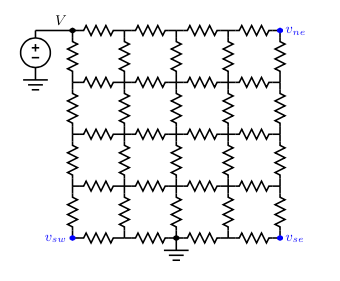
\includegraphics[scale =0.6 ]{./sample1.png}
\section{Implementation of Power Methods}
\begin{description}  

\item [Power Method:] For power method, I perform the following process iteratively until the accuracy reaches the requirements, that is, the process ends when the accuracy I set reaches $10^{-9}$.  $\nu$ is supposed to be maximal eigenvalue in this method.\\
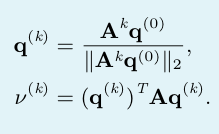
\includegraphics[scale =0.6 ]{./power_method.png}\\

\item [Inverse Power Method:] I implemented the following method and let it run iteratively. The requirement is the same as power method. $z$ can be calculated by LU method in the first formula and $\mu$ should be desired minimal eigenvalue in the end.\\
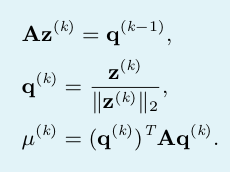
\includegraphics[scale =0.6 ]{./inverse_power.png}\\

\item [Ending condition:] For the power method and its inverse form, I use the following RHS as the criteria. When it becomes smaller than $10^{-9}$, the function would terminate.\\
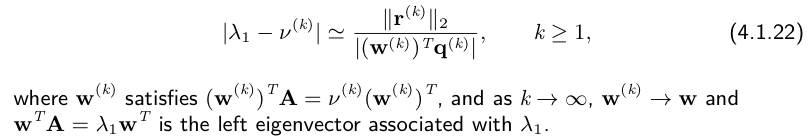
\includegraphics[scale =0.6 ]{./stopping_criteria.png}\\

\end{description}

\section{Workflow}

\begin{description}  

\item [Usage:] For example, ./hw07.out $num$. $num$ is the number of resisters per side. $num = 2, 4, 10, 20, 40$.
%one in HW04 and the default resistance is $100Ohms$.
\item [Form matrix:] For linear system like the above figure, first build system matrix $A$ with Kirchoff node method.
\item [Modify matrix:] Modify matrix $A$ to be a symmetric matrix. 
%\item [Initialize RHS:] Since LHS is modified, RHS shall simultaneously be assigned accordingly so that the linear system stay equivalent to the original one.
\item [Solve:] Use Power method and Inverse Power Method to get the largest and the smallest eigenvalues and then calculate the condition number.
\item[Desired output format:] You should be able to see results of $lambda_{max}$, $lambda_{min}$ and the condition number in a row. Note: for symmetric and positive definite matrix, $lambda_{max}$ and $lambda_{min}$ are equivalent to $lambda_{1}$ and $lambda_{n}$.
\end{description}

\section{Results}

\begin{tabular}{|c|c|c|c|c|}
\hline  Resistors Per Side & condition number  &  $lambda_{max}$   & $lambda_{min}$ &  Time(s)  \\
\hline    2    			& 1849.470024 	& 1 		& 5.406954e-4 	& 0.0010    \\

\hline    4    			& 3607.461004 	& 1		 & 2.772033e-4  & 0     \\
\hline    10  			& 10653.368024 	& 1 		& 9.386703e-5 	& 0.0230      \\

\hline    20  			& 25212.310283 	& 1		& 3.966316e-5 	&  0.6360      \\

\hline    40  			& 59700.888558   	& 1		& 1.675017e-5	 &31.5630    \\\hline 
\end{tabular}

\section{Plot Analysis}
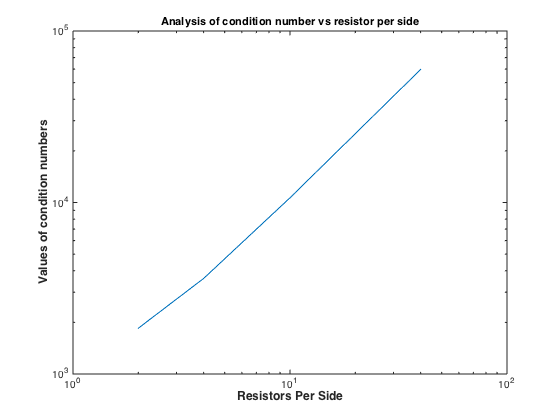
\includegraphics[scale =0.7 ]{./condition_number.png}\\
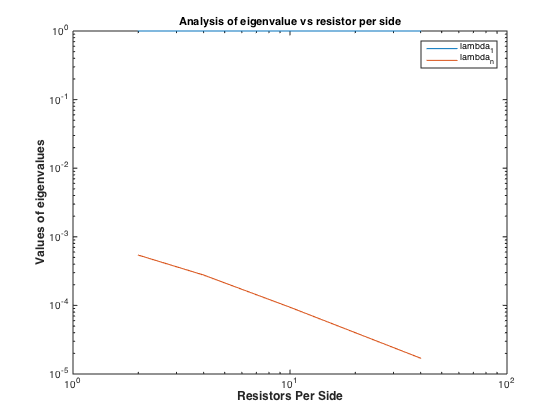
\includegraphics[scale =0.75]{./eigenvalues.png}\\
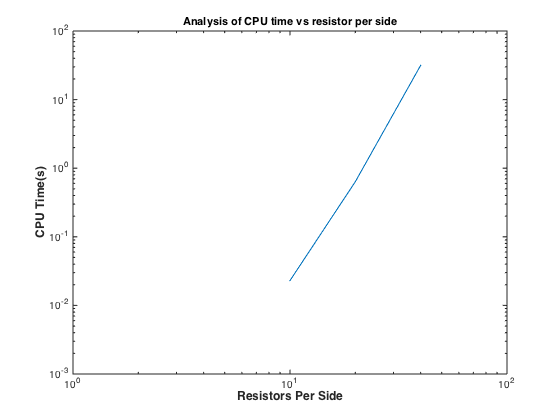
\includegraphics[scale =0.75]{./CPUtime.png}\\

\section{Observations}

\begin{description}

\item [CPU time:]  Overall complexity of HW7 is roughly $O(n^{2.91})$, derived from $\frac{log(31.5630) - log(0.6360)}{log((40+1)^2) - log((20+1)^2)}$. Since in inverse power method, it is necessary to use LU decomposition to get a intermediate term and LU method is about $O(n^3)$, so LU method will dominate the complexity. It is not guaranteed to directly find complexity of power method by observation in this assignment except we separately measure the time of power method phase and inverse power method phase, but that is not the main purpose of this assignment.

\item [Eigenvalues:] The smallest eigenvalue tends to exponentially decay as the matrix size expands. The largest eigenvalue maintains to be $1$ all the way. 

\item [Condition number:] The condition number ascends exponentially as the resistors per side doubles which means as the matrix size getting larger, the numerical solution of the system is getting way more inaccurate. 

\item [Accuracy:] In my program, I use the following equation as my stopping criteria. Therefore, if the RHS is smaller than $10^{-9}$, then my result is extremely close to the true eigenvalue.\\
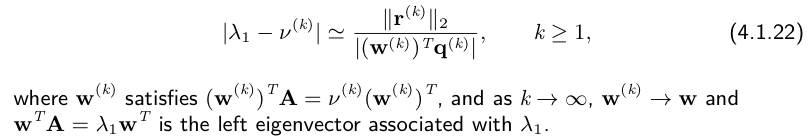
\includegraphics[scale =0.5]{./stopping_criteria.png}\\

\item[Overall:] The overall process for finding condition number works pretty well since the time required to get the result is fast enough to me. So, power method and its inverse form are both very good iterative method.


\end{description}


\end{document} 